\documentclass[11pt,a4paper]{article}

\usepackage[margin=2.5cm]{geometry}
\usepackage[T1]{fontenc}
\usepackage[utf8]{inputenc}
\usepackage{lmodern}
\usepackage{amsmath,amssymb}
\usepackage{booktabs}
\usepackage{array}
\usepackage{tabularx}
\usepackage{longtable}
\usepackage{graphicx}
\usepackage{xcolor}
\usepackage{float}
\usepackage{enumitem}
\usepackage{url}
\usepackage{hyperref}
\usepackage{caption}
\usepackage{subcaption}
\usepackage{microtype}
\usepackage{placeins}

\graphicspath{{figures/}}
\hypersetup{
  colorlinks=true,
  linkcolor=blue,
  citecolor=blue,
  urlcolor=blue,
  pdfauthor={24376333 Huang Yibo; 24376267 Wang Xihao; 24301017 Yang Xiaochu},
  pdftitle={A Comparative Study of ORB-Style, DSO-Style, and SVO-Style Visual SLAM Baselines on KITTI}
}
\urlstyle{same}
\sloppy

\newcolumntype{Y}{>{\raggedright\arraybackslash}X}
\newcommand{\NA}{\textsc{N/A}}
\newcommand{\paperclaim}{\texttt{implementation\_manifest.paper\_level\_claim=false}}
\newcommand{\methodorb}{ORB-SLAM2-inspired stereo SLAM}
\newcommand{\methoddso}{DSO-inspired direct sparse stereo SLAM}
\newcommand{\methodsvo}{SVO-style semi-direct stereo visual odometry/SLAM}

\title{A Comparative Study of ORB-Style, DSO-Style, and SVO-Style Visual SLAM Baselines on KITTI}
\author{\large\bfseries 24376333 Huang Yibo \quad 24376267 Wang Xihao \quad 24301017 Yang Xiaochu\\[0.3em]
Machine Learning Course Project}
\date{\today}

\begin{document}
\maketitle

\section{Title}

The title of this report is \emph{A Comparative Study of ORB-Style, DSO-Style, and SVO-Style Visual SLAM Baselines on KITTI}. The report evaluates three reproducible Python research baselines inspired by classical visual SLAM systems: \methodorb{}, \methoddso{}, and \methodsvo{}. The central goal is to compare feature-based, direct sparse, and semi-direct visual SLAM/VO designs under a unified benchmark protocol on KITTI Odometry sequence 00.

The final version of the report uses the latest completed 300-frame experiment with 800 ORB features or sparse points per method. The strongest overall speed-accuracy trade-off is obtained by the SVO-style baseline, while the ORB-style baseline remains highly robust and the optimized DSO-style baseline becomes substantially more competitive than the earlier simplified direct sparse result. The analysis emphasizes not only ATE RMSE, but also RPE, KITTI-style segment metrics, runtime, keyframe behavior, tracking failures, fallback events, loop-candidate semantics, and DSO diagnostic counters.

The report deliberately avoids overclaiming. The implemented systems are reproducible Python research baselines inspired by classical SLAM systems, not official ORB-SLAM2, DSO, or SVO implementations and not complete paper-level reproductions. The project manifest explicitly states \paperclaim{}.

\section{Background and Significance}

Simultaneous localization and mapping (SLAM) is a fundamental problem in mobile robotics and autonomous driving. A SLAM system estimates the trajectory of a moving sensor platform while maintaining geometric information about the surrounding environment. Visual SLAM is especially important because cameras are low-cost, compact, and information-rich sensors. In a stereo setting, image texture and calibrated disparity provide both appearance cues and metric depth cues, which makes stereo visual odometry suitable for vehicle-scale trajectory estimation on datasets such as KITTI Odometry.

The practical difficulty is that visual SLAM is not a single algorithmic problem. It is an interaction between visual correspondence, depth initialization, pose estimation, outlier rejection, map maintenance, and backend optimization. Illumination variation, repeated structures, motion blur, low texture, moving objects, calibration errors, and imperfect point lifecycles can all produce wrong correspondences or unstable residuals. Therefore, a useful course project should not only report a final number, but also expose why a method succeeds or fails under a controlled protocol.

Classical visual SLAM and visual odometry systems are commonly grouped into three families. Feature-based systems detect repeatable keypoints and match descriptors before estimating motion geometrically. Direct sparse systems avoid descriptor matching and instead optimize photometric residuals over selected pixels. Semi-direct systems retain sparse map geometry but track points using patch alignment or optical flow. These families make different engineering trade-offs. Feature-based pipelines often gain robustness from explicit matching and RANSAC, but descriptor extraction and local map operations can be expensive. Direct pipelines can use lower-level image information, but their optimization is sensitive to initialization and photometric assumptions. Semi-direct pipelines can reduce matching cost while retaining sparse geometric pose estimation.

The significance of this project is that it implements all three families inside one Python framework. All methods use the same KITTI stereo input, calibration interface, trajectory output format, origin alignment setting, evaluation script, and JSON reporting schema. This makes the comparison controlled at the project level. At the same time, because the three baselines do not have the maturity of their official C++ counterparts, the results should be interpreted as evidence about implementation-level behavior rather than universal claims about algorithm families.

This report addresses three research questions:
\begin{enumerate}[leftmargin=2em]
  \item Under the same KITTI sequence, frame count, alignment setting, and evaluation code, how do the three Python baselines differ in trajectory accuracy, segment error, runtime, and robustness?
  \item Does the SVO-style semi-direct baseline provide a measurable speed-accuracy compromise between descriptor-based tracking and direct sparse tracking?
  \item Which implementation factors explain the remaining failures of the optimized DSO-style baseline, and how do active-window BA, left-right stereo consistency, quality gates, residual filtering, and fallback policies affect the final result?
\end{enumerate}

\section{Literature Review}

\subsection{Feature-Based Visual SLAM}

Feature-based visual SLAM converts images into sparse keypoints and descriptors. Camera motion is then estimated from feature correspondences using geometric verification, triangulation, PnP, and bundle adjustment. ORB-SLAM2 is a representative feature-based SLAM system for monocular, stereo, and RGB-D cameras. It combines ORB features, keyframe-based mapping, local bundle adjustment, relocalization, and loop closing \cite{mur2017orbslam2}. The ORB feature itself was designed as an efficient alternative to SIFT and SURF and remains widely used in real-time visual systems \cite{rublee2011orb}.

The main strength of feature-based SLAM is that its correspondences have explicit geometric meaning. Outlier rejection can be performed before pose optimization using RANSAC, and local map tracking can reuse stable map points across frames. This explains why feature-based systems often remain robust when repeatable texture is available. The main costs are descriptor extraction, descriptor matching, map-point management, and local optimization. In this project, the ORB-style baseline implements stereo depth, ORB feature extraction, PnP RANSAC, keyframes, sparse map points, and loop-count statistics. It does not reproduce the full official ORB-SLAM2 backend, vocabulary behavior, or production-level runtime.

\subsection{Direct Sparse Odometry}

Direct sparse methods avoid explicit descriptor matching and instead optimize intensity residuals. Direct Sparse Odometry (DSO) selects high-gradient pixels and jointly optimizes camera poses, inverse depths, and photometric parameters in a sparse direct formulation \cite{engel2018dso}. Full DSO depends on calibrated photometric response handling, sparse direct bundle adjustment, active-window marginalization, and carefully maintained point lifecycles.

The advantage of a direct sparse formulation is that it can use image information that may not be captured by discrete descriptors. However, this advantage comes with stricter assumptions. Brightness constancy can be violated by exposure changes, non-Lambertian surfaces, shadows, and camera response effects. The photometric objective is also nonconvex, so an inaccurate initial pose can move the optimizer toward poor local minima. As a result, simplified DSO-style implementations require strong safeguards: good initialization, spatially uniform point selection, residual filtering, motion gates, and fallback logic. The \methoddso{} in this project uses stereo initialization, high-gradient sparse points, an inverse-depth active window, LK+PnP initialization, simplified photometric refinement, affine brightness handling, left-right stereo consistency, active-window BA counters, strict loop verification semantics, and per-frame diagnostics. It remains a Python research baseline rather than a complete reproduction of the original DSO system.

\subsection{Semi-Direct Visual Odometry}

SVO introduced a semi-direct visual odometry design that combines sparse map structure with direct image alignment \cite{forster2014svo}. The central idea is to avoid expensive descriptor matching during normal frame-to-frame tracking while still preserving sparse geometric constraints. A semi-direct system commonly tracks projected map points using patch alignment or optical flow and then estimates the camera pose using geometric constraints.

The SVO-style baseline in this project follows that principle. It uses grid-uniform sparse point selection, stereo depth initialization, pyramidal Lucas-Kanade optical flow for patch-level tracking, PnP RANSAC for 3D-2D pose estimation, and keyframe refresh for local map maintenance. Lucas-Kanade tracking provides a classical basis for iterative image registration \cite{lucas1981iterative}, while RANSAC provides robust model selection when some tracked correspondences are outliers \cite{fischler1981random}. The implementation does not include the full SVO probabilistic depth filter, mature backend, production relocalization, or loop closure.

\subsection{KITTI and Modern Deep SLAM}

The KITTI Vision Benchmark Suite provides outdoor driving datasets and benchmark tasks for stereo vision, optical flow, visual odometry, SLAM, and related autonomous-driving problems \cite{geiger2012kitti}. This project uses KITTI Odometry sequence 00 because it provides calibrated stereo images and a ground-truth trajectory suitable for controlled VO/SLAM evaluation.

Modern learning-based systems such as DROID-SLAM and DPVO combine neural matching or neural update mechanisms with differentiable optimization \cite{teed2021droidslam,teed2023dpvo}. They are important related work, but they require pretrained models and a different engineering stack. Since this project is an implementation-oriented comparison of classical Python baselines, deep SLAM systems are discussed as context rather than included as primary experimental algorithms.

\section{Methodological Principles}

\subsection{Unified Benchmark Framework}

All three methods use the same KITTI stereo loader, calibration data, trajectory format, evaluation script, and JSON reporting logic. Each input frame must produce one $4\times4$ pose matrix. When a tracker fails, the system must still keep the trajectory length unchanged by using fallback or a previous safe pose. Failed frames are not removed, and trajectories are not silently truncated. This fairness control is essential because dropping failed frames would artificially favor unstable methods.

Figure~\ref{fig:workflow} shows the shared workflow. The ORB-style frontend uses feature matching and geometric pose estimation. The DSO-style frontend uses sparse photometric residuals after LK+PnP initialization. The SVO-style frontend uses patch or optical-flow tracking followed by PnP. The shared output layer writes trajectory files, benchmark JSON, trajectory plots, and diagnostic plots.

\begin{figure}[H]
  \centering
  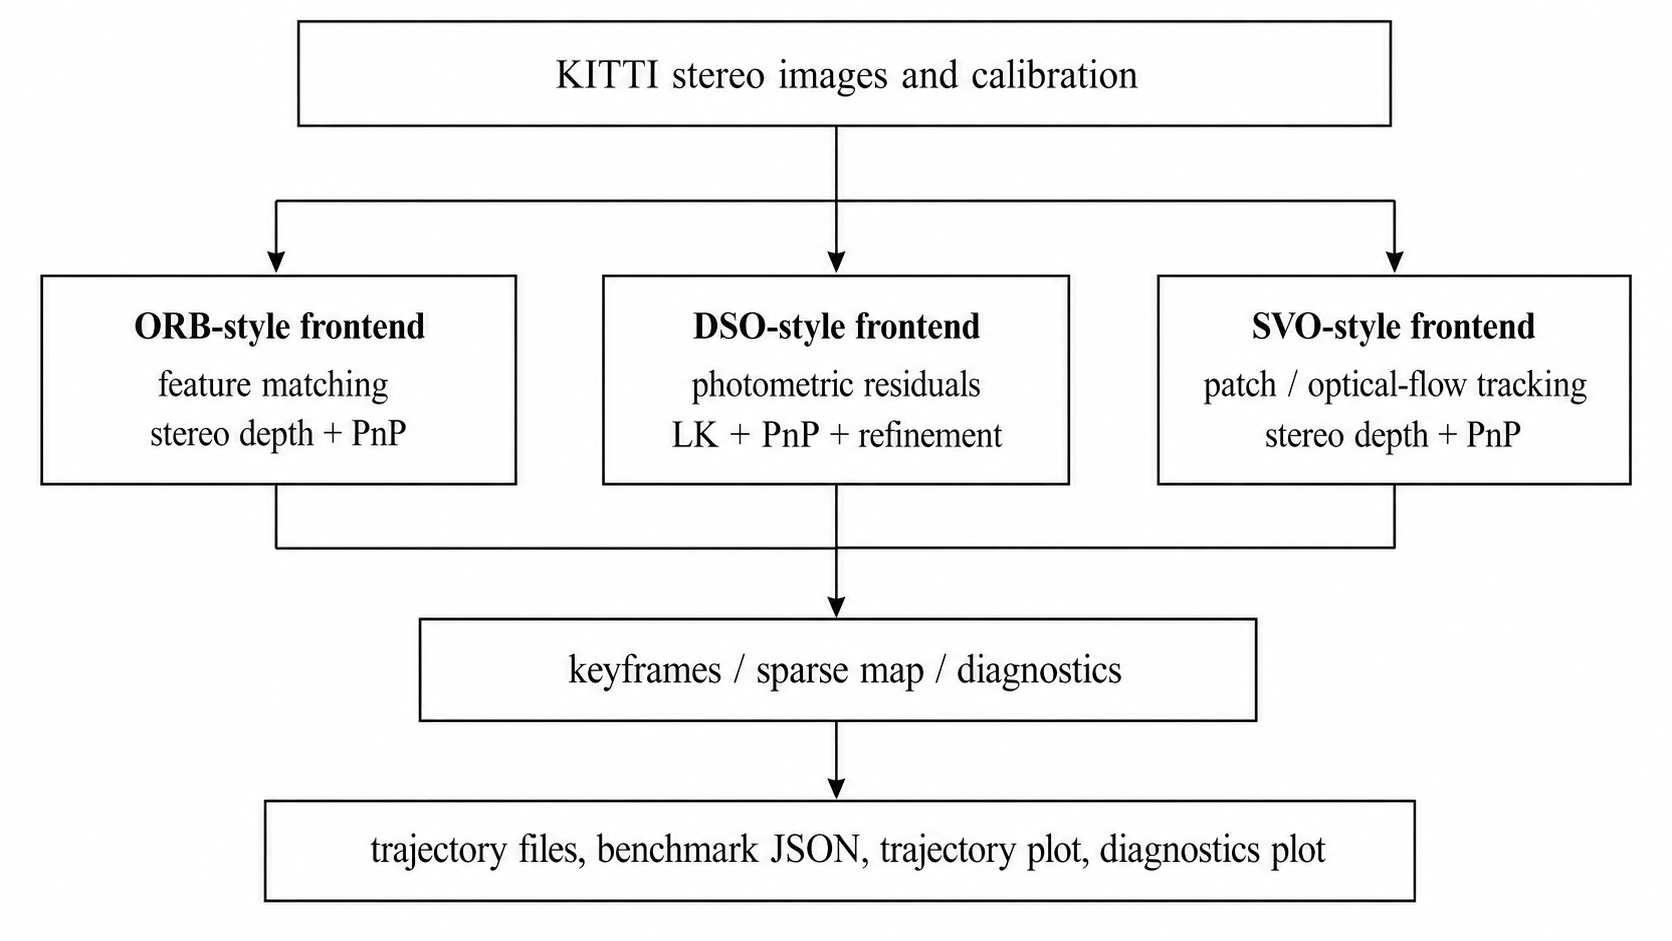
\includegraphics[width=0.92\textwidth]{Workflow.png}
  \caption{Shared benchmark workflow for the three Python SLAM/VO baselines.}
  \label{fig:workflow}
\end{figure}

\subsection{ORB-SLAM2-Inspired Stereo SLAM}

The \methodorb{} baseline detects ORB features in stereo images and initializes sparse metric 3D points from stereo disparity. The current-frame pose is estimated from correspondences between local 3D map points and 2D feature observations. PnP with RANSAC rejects inconsistent matches before accepting a pose. New keyframes are inserted when tracking quality, parallax, or motion thresholds indicate that the local map should be refreshed.

The geometric pose estimation problem can be written as robust reprojection-error minimization:
\begin{equation}
  \min_{T\in SE(3)} \sum_{i\in\mathcal{I}} \rho\left(\left\|u_i - \pi(TP_i)\right\|_2^2\right),
\end{equation}
where $P_i$ is a 3D map point, $u_i$ is its current 2D observation, $\pi(\cdot)$ is the calibrated camera projection function, $T$ is the current pose, and $\rho$ denotes either a robust loss or the inlier set selected by RANSAC.

This design explains the experimental behavior observed later. RANSAC and local map reuse make the ORB-style baseline robust to individual mismatches, and the final 300-frame run records zero tracking failures. The cost is that feature extraction, matching, local map tracking, and occasional loop-related checks create a heavy-tailed runtime distribution in Python.

\subsection{DSO-Inspired Direct Sparse Stereo SLAM}

The \methoddso{} baseline selects sparse high-gradient locations with valid stereo depth. For a reference image $I_r$ and current image $I_t$, the photometric residual for a sparse 3D point $P_i$ can be expressed as
\begin{equation}
  r_i(\xi) = I_t\left(\pi(\exp(\xi)P_i)\right) - I_r(u_i),
\end{equation}
where $\xi$ is a pose increment in the Lie algebra of $SE(3)$. The simplified direct objective is
\begin{equation}
  E_{\mathrm{photo}}(\xi) = \sum_{i\in\Omega}\rho\left(r_i(\xi)^2\right),
\end{equation}
where $\Omega$ is the set of sparse points that can be validly projected into the current frame.

The optimized DSO configuration used in the final 300-frame run enables grid-uniform point selection, left-right stereo depth consistency, affine brightness compensation, residual filtering, low valid-projection rejection, motion gates, cost-jump gates, active-window BA, strict loop verification, and fallback. When a candidate pose is rejected, the system falls back to LK+PnP, constant velocity, or the previous safe pose. Per-frame diagnostics record tracking cost, valid projected points, residual mean, residual median, residual 95th percentile, inlier ratio, relative motion, fallback reason, keyframe insertion, active inverse-depth points, point culling, BA counters, and loop-candidate counters.

The method-design implication is direct. Photometric residuals can make efficient use of sparse image information, but they are sensitive to initialization, brightness changes, residual outliers, and point lifecycle errors. Therefore, the final DSO result should be judged together with diagnostics and ablations rather than by ATE alone.

\subsection{SVO-Style Semi-Direct Stereo Visual Odometry/SLAM}

The \methodsvo{} baseline lies between the feature-based and direct sparse pipelines. It does not rely on ORB descriptor matching as its primary tracking mechanism. Instead, sparse points from a reference keyframe are tracked in the current frame using pyramidal Lucas-Kanade optical flow or patch-level alignment. The tracked 2D locations are paired with reference-frame 3D points, and \texttt{solvePnPRansac} estimates the current pose from these 3D-2D correspondences.

This design preserves stereo depth initialization and geometric verification while avoiding the cost of full descriptor matching in every frame. Keyframe insertion is triggered by tracked point count, PnP inlier ratio, parallax, translation, rotation, or elapsed frames since the last keyframe. The reported SVO-style baseline records keyframes, active sparse points, tracking failures, fallback count, loop-closure status, mean tracked points, and mean PnP inliers.

The design also explains the final runtime result. Optical-flow tracking is lighter than descriptor matching, and the PnP stage still provides geometric robustness. The trade-off is that this baseline has no production-grade loop closure and inserts many keyframes to maintain a fresh local reference.

\subsection{Evaluation Metrics and Fairness Controls}

The main trajectory metric is origin-aligned absolute trajectory error (ATE) RMSE:
\begin{equation}
  \mathrm{ATE}_{\mathrm{RMSE}} = \sqrt{\frac{1}{N}\sum_{i=1}^{N}\left\|\mathrm{trans}\left((T_i^{\mathrm{gt}})^{-1}AT_i^{\mathrm{est}}\right)\right\|_2^2},
\end{equation}
where $T_i^{\mathrm{gt}}$ is the ground-truth pose, $T_i^{\mathrm{est}}$ is the estimated pose, and $A$ is the alignment transform. The benchmark also stores relative pose error (RPE), KITTI-style segment metrics, runtime average/median/95th percentile, wall time, keyframe count, tracking failures, fallbacks, loop closures, and method-specific robustness statistics.

Fairness controls include the same KITTI sequence, the same 300-frame input limit, the same origin alignment, the same trajectory output format, the same evaluation code, and strict trajectory-length checking. All JSON outputs are standard JSON; non-finite values such as NaN and infinity are converted to \texttt{null}. In the 300-frame run, KITTI-style 100 m and 200 m segment metrics are available, while 300 m to 800 m segments remain unavailable because the selected subsequence is shorter than those path lengths. Segment means are computed over the available lengths only.

\section{Experimental Results and Analysis}

\subsection{Experimental Setup}

The final main experiment uses the first 300 frames of KITTI Odometry sequence 00. The selected output directory is
\begin{center}
\texttt{results/final\_seq00\_300\_optimized\_f800\_p800}.
\end{center}
The configuration is: ORB features = 800, DSO points = 800, SVO points = 800, and alignment = origin. The DSO main configuration is the optimized strict configuration with grid selection, left-right depth consistency, outlier handling, motion gates, cost-jump rejection, photometric refinement, affine brightness handling, strict loop verification, active-window BA, and fallback mode set to LK+PnP followed by constant velocity if needed. All three methods output 300 poses.

Runtime values are local measurements on the same workstation rather than hardware-normalized performance claims, because detailed hardware specifications were not logged. A previous 100-frame report used a shorter final benchmark; the present version supersedes it with the completed 300-frame run and optimized DSO diagnostics.

Table~\ref{tab:components} summarizes the implemented components and omitted full-system components. This distinction is necessary because the three baselines differ in backend maturity. The comparison is a project-level baseline comparison, not a ranking of the full official systems.

\begin{table}[H]
\centering
\scriptsize
\caption{Implemented components and known omissions of the three visual SLAM/VO baselines.}
\label{tab:components}
\begin{tabularx}{\textwidth}{p{0.16\textwidth}YYY}
\toprule
Category & ORB-SLAM2-inspired stereo SLAM & DSO-inspired direct sparse stereo SLAM & SVO-style semi-direct stereo visual odometry/SLAM \\
\midrule
Frontend & ORB feature extraction, sparse matching, and geometric verification & High-gradient sparse points, photometric residuals, and LK+PnP initialization & Grid-uniform sparse points with patch/optical-flow tracking \\
Depth initialization & Stereo disparity and metric depth & Stereo depth, left-right consistency, and inverse-depth active points & Stereo depth initialization for reference sparse points \\
Pose estimation & 3D-2D PnP RANSAC and local tracking & LK+PnP plus simplified photometric refinement and active-window BA & Optical-flow tracks plus 3D-2D PnP RANSAC \\
Keyframes and map & Keyframes, map points, and local mapping structures & Active keyframe window, inverse-depth points, marginalization counters, and point culling & Keyframes, active sparse points, and local map refresh \\
Robustness & Tracking-failure statistics, relocalization statistics, and loop-count statistics & Motion gates, quality gates, outlier handling, fallback, strict loop verification, and per-frame diagnostics & Motion gate, PnP inlier filtering, fallback, and loop-disabled reporting \\
Missing full-system components & Full official ORB-SLAM2 maturity, large-scale vocabulary behavior, and complete production backend & Full original DSO photometric BA, calibrated response/exposure/vignetting model, complete Schur-complement marginalization, and mature point lifecycle & Full SVO probabilistic depth filter, mature backend, production relocalization, and loop closure \\
\bottomrule
\end{tabularx}
\end{table}

\subsection{Main 300-Frame Results}

Table~\ref{tab:main-results} reports the final 300-frame accuracy comparison. The SVO-style baseline obtains the lowest ATE RMSE, 2.9621 m, and also has the lowest translational RPE and KITTI mean translational segment error. The ORB-style baseline is close in ATE, with 2.9913 m and zero tracking failures. The optimized DSO-style baseline obtains 3.4279 m ATE RMSE. This is higher than ORB and SVO in global ATE, but it is much closer to the other two baselines than in the earlier simplified DSO result. DSO also has lower translational RPE and segment translational error than ORB in this run, which shows why the result should not be reduced to a single metric.

\begin{table}[H]
\centering
\small
\caption{Main 300-frame accuracy results on KITTI sequence 00. Configuration: origin alignment, 800 ORB features, 800 DSO points, and 800 SVO points. KITTI mean values are computed over the available 100 m and 200 m segments.}
\label{tab:main-results}
\begin{tabular}{lccccc}
\toprule
Algorithm & ATE RMSE (m) & RPE t (\%) & RPE r (deg/m) & KITTI t (\%) & KITTI r (deg/m) \\
\midrule
ORB & 2.9913 & 2.7487 & 0.02778 & 2.6843 & 0.02646 \\
DSO & 3.4279 & 2.0376 & 0.01598 & 2.0259 & 0.01543 \\
SVO & 2.9621 & 1.7526 & 0.01807 & 1.7257 & 0.01730 \\
\bottomrule
\end{tabular}
\end{table}

Table~\ref{tab:runtime} reports runtime and robustness. SVO is the fastest baseline by a large margin, with an average runtime of 39.64 ms per frame and wall time of 13.59 s. ORB is the slowest in this Python implementation, and the gap between its median runtime and p95 runtime indicates a heavy-tailed computation pattern. DSO is between ORB and SVO, but it records 12 failures and 12 fallbacks.

\begin{table}[H]
\centering
\small
\caption{Runtime and robustness summary for the final 300-frame run. Runtime values are local Python measurements and are not hardware-normalized.}
\label{tab:runtime}
\resizebox{\textwidth}{!}{%
\begin{tabular}{lccccc}
\toprule
Algorithm & Runtime avg/med/p95 (ms) & Wall time (s) & Keyframes & Failures / fallbacks & Loop candidates / closures \\
\midrule
ORB & 5239.21 / 31.29 / 26338.86 & 1575.81 & 103 & 0 / \NA{} & 89 / 2 \\
DSO & 1759.10 / 129.18 / 10269.94 & 527.78 & 141 & 12 / 12 & 17 / 0 \\
SVO & 39.64 / 47.13 / 64.01 & 13.59 & 217 & 0 / 0 & 0 / 0 \\
\bottomrule
\end{tabular}}
\end{table}

Table~\ref{tab:segments} reports the available KITTI-style segment metrics. The 300-frame subsequence provides 158 segments of approximately 100 m and 19 segments of approximately 200 m, for 177 valid segment measurements. Longer lengths are not available and are therefore omitted rather than imputed.

\begin{table}[H]
\centering
\small
\caption{Available KITTI-style segment metrics for the final 300-frame run. Each cell reports translational error in percent and rotational error in deg/m.}
\label{tab:segments}
\resizebox{\textwidth}{!}{%
\begin{tabular}{lcccc}
\toprule
Algorithm & 100 m t/r & 200 m t/r & Valid segments & Mean t/r \\
\midrule
ORB & 2.7487 / 0.02778 & 2.1492 / 0.01549 & 177 & 2.6843 / 0.02646 \\
DSO & 2.0376 / 0.01598 & 1.9280 / 0.01086 & 177 & 2.0259 / 0.01543 \\
SVO & 1.7526 / 0.01807 & 1.5021 / 0.01094 & 177 & 1.7257 / 0.01730 \\
\bottomrule
\end{tabular}}
\end{table}

Figure~\ref{fig:traj-zoom} shows the trajectory comparison and a zoomed crop of the turn section. The three estimates follow the same main route. In the zoomed view, the SVO-style and ORB-style estimates remain close in global shape, while the optimized DSO-style trajectory is also much more stable than the earlier direct sparse baseline. The plot should be interpreted together with Tables~\ref{tab:main-results} and~\ref{tab:runtime}: SVO has the best ATE and runtime, ORB has zero failures and two loop closures, and DSO has competitive segment errors but more failure events.

\begin{figure}[H]
  \centering
  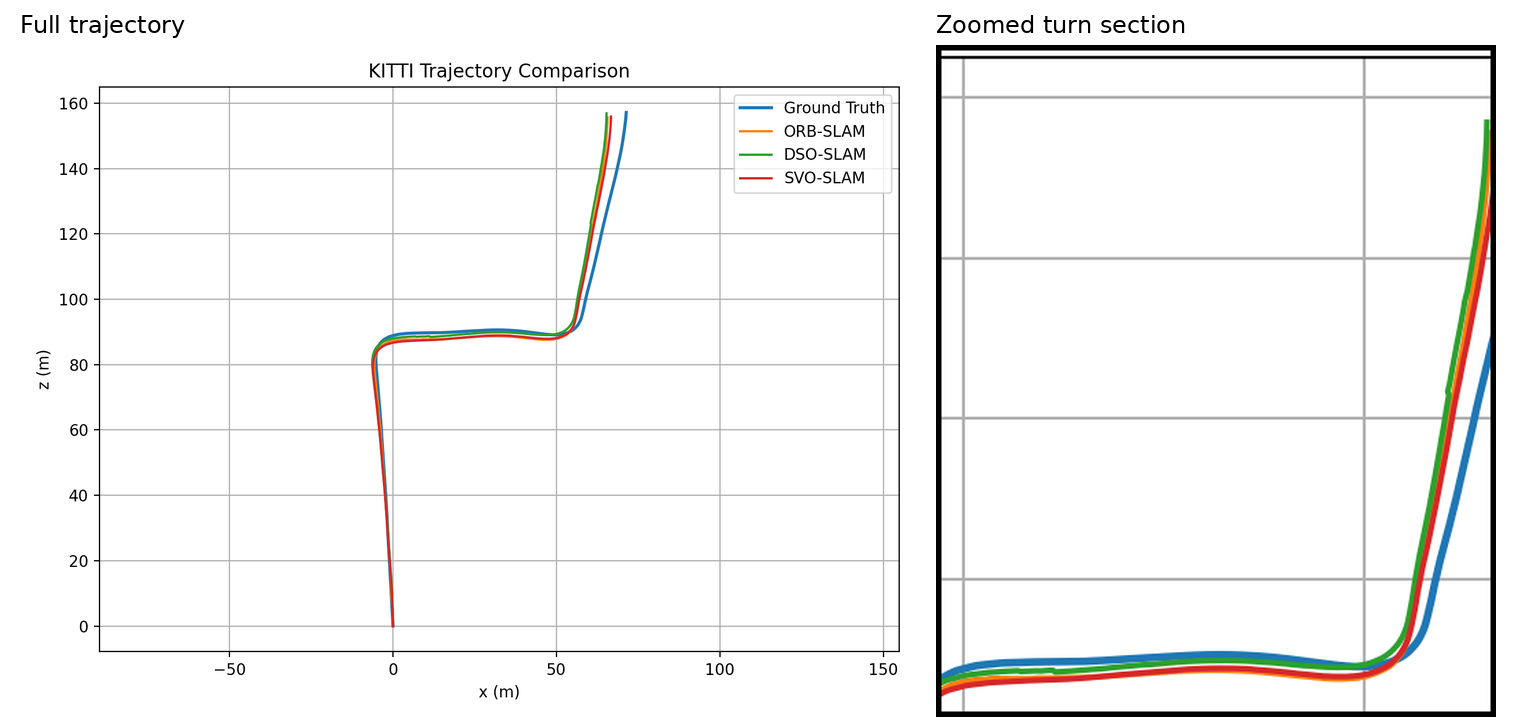
\includegraphics[width=\textwidth]{final300_trajectory_with_zoom.png}
  \caption{Trajectory comparison for the first 300 frames of KITTI sequence 00, with a zoomed crop of the turn section. The full plot is the benchmark-generated trajectory figure; the zoom panel is a crop of the same figure for readability.}
  \label{fig:traj-zoom}
\end{figure}

\FloatBarrier

\subsection{Robustness and DSO Diagnostics}

Table~\ref{tab:diagnostics} summarizes robustness statistics for the final 300-frame run. The optimized DSO-style baseline processes all 300 frames and records 12 tracking failures with 12 fallbacks. Ten fallbacks use LK+PnP, and two use constant velocity. The failure frames are 20, 71, 75, 112, 137, 144, 185, 210, 247, 253, 259, and 276. The maximum relative translation is 5.3400 m, and the maximum relative rotation is 4.0301 degrees. The DSO implementation also records 17 loop candidates but zero verified loop closures and zero loop corrections, which avoids treating candidate loops as actual closures.

\begin{table}[H]
\centering
\scriptsize
\caption{Robustness and DSO diagnostics summary for the final 300-frame run. DSO residual statistics are computed from \texttt{dso\_diagnostics\_seq00.json}.}
\label{tab:diagnostics}
\begin{tabular}{lccc}
\toprule
Statistic & ORB & DSO & SVO \\
\midrule
Frames processed & 300 & 300 & 300 \\
Keyframes & 103 & 141 & 217 \\
Tracking failures & 0 & 12 & 0 \\
Fallbacks & \NA{} & 12 & 0 \\
Motion gate rejections & \NA{} & 2 & 0 \\
Cost-jump rejections & \NA{} & 1 & \NA{} \\
Loop candidates & 89 & 17 & 0 \\
Verified/applied loop closures & 2 & 0 & 0 \\
Mean valid projected/tracked points & \NA{} & 629.66 & 535.76 \\
Median valid projected/tracked points & \NA{} & 654.00 & 549.00 \\
Mean inlier ratio & \NA{} & 0.7248 & 0.7645 \\
Mean PnP inliers & \NA{} & \NA{} & 413.57 \\
Mean residual mean & \NA{} & 22.0511 & \NA{} \\
Median residual median & \NA{} & 11.6218 & \NA{} \\
Mean residual p95 & \NA{} & 74.7853 & \NA{} \\
Median residual p95 & \NA{} & 73.1055 & \NA{} \\
Max relative translation (m) & \NA{} & 5.3400 & \NA{} \\
Max relative rotation (deg) & \NA{} & 4.0301 & \NA{} \\
BA accepted / runs / rejected & \NA{} & 47 / 64 / 17 & \NA{} \\
Active sparse/inverse-depth points & 17534 & 2998 & 3879 \\
Active DSO points culled & \NA{} & 1282 & \NA{} \\
Stereo depth filtering & \NA{} & left-right consistency & \NA{} \\
\bottomrule
\end{tabular}
\end{table}

Figure~\ref{fig:dso-diagnostics-enhanced} visualizes valid projected points, photometric inlier ratio, residual statistics, and the distribution of residual 95th percentiles. Red vertical markers denote failure/fallback frames. The failures are sparse rather than one long continuous collapse. Several failure markers coincide with lower valid projection counts, lower inlier ratios, or higher residual percentiles, supporting the interpretation that remaining DSO instability is associated with residual-set quality and local tracking conditions.

\begin{figure}[H]
  \centering
  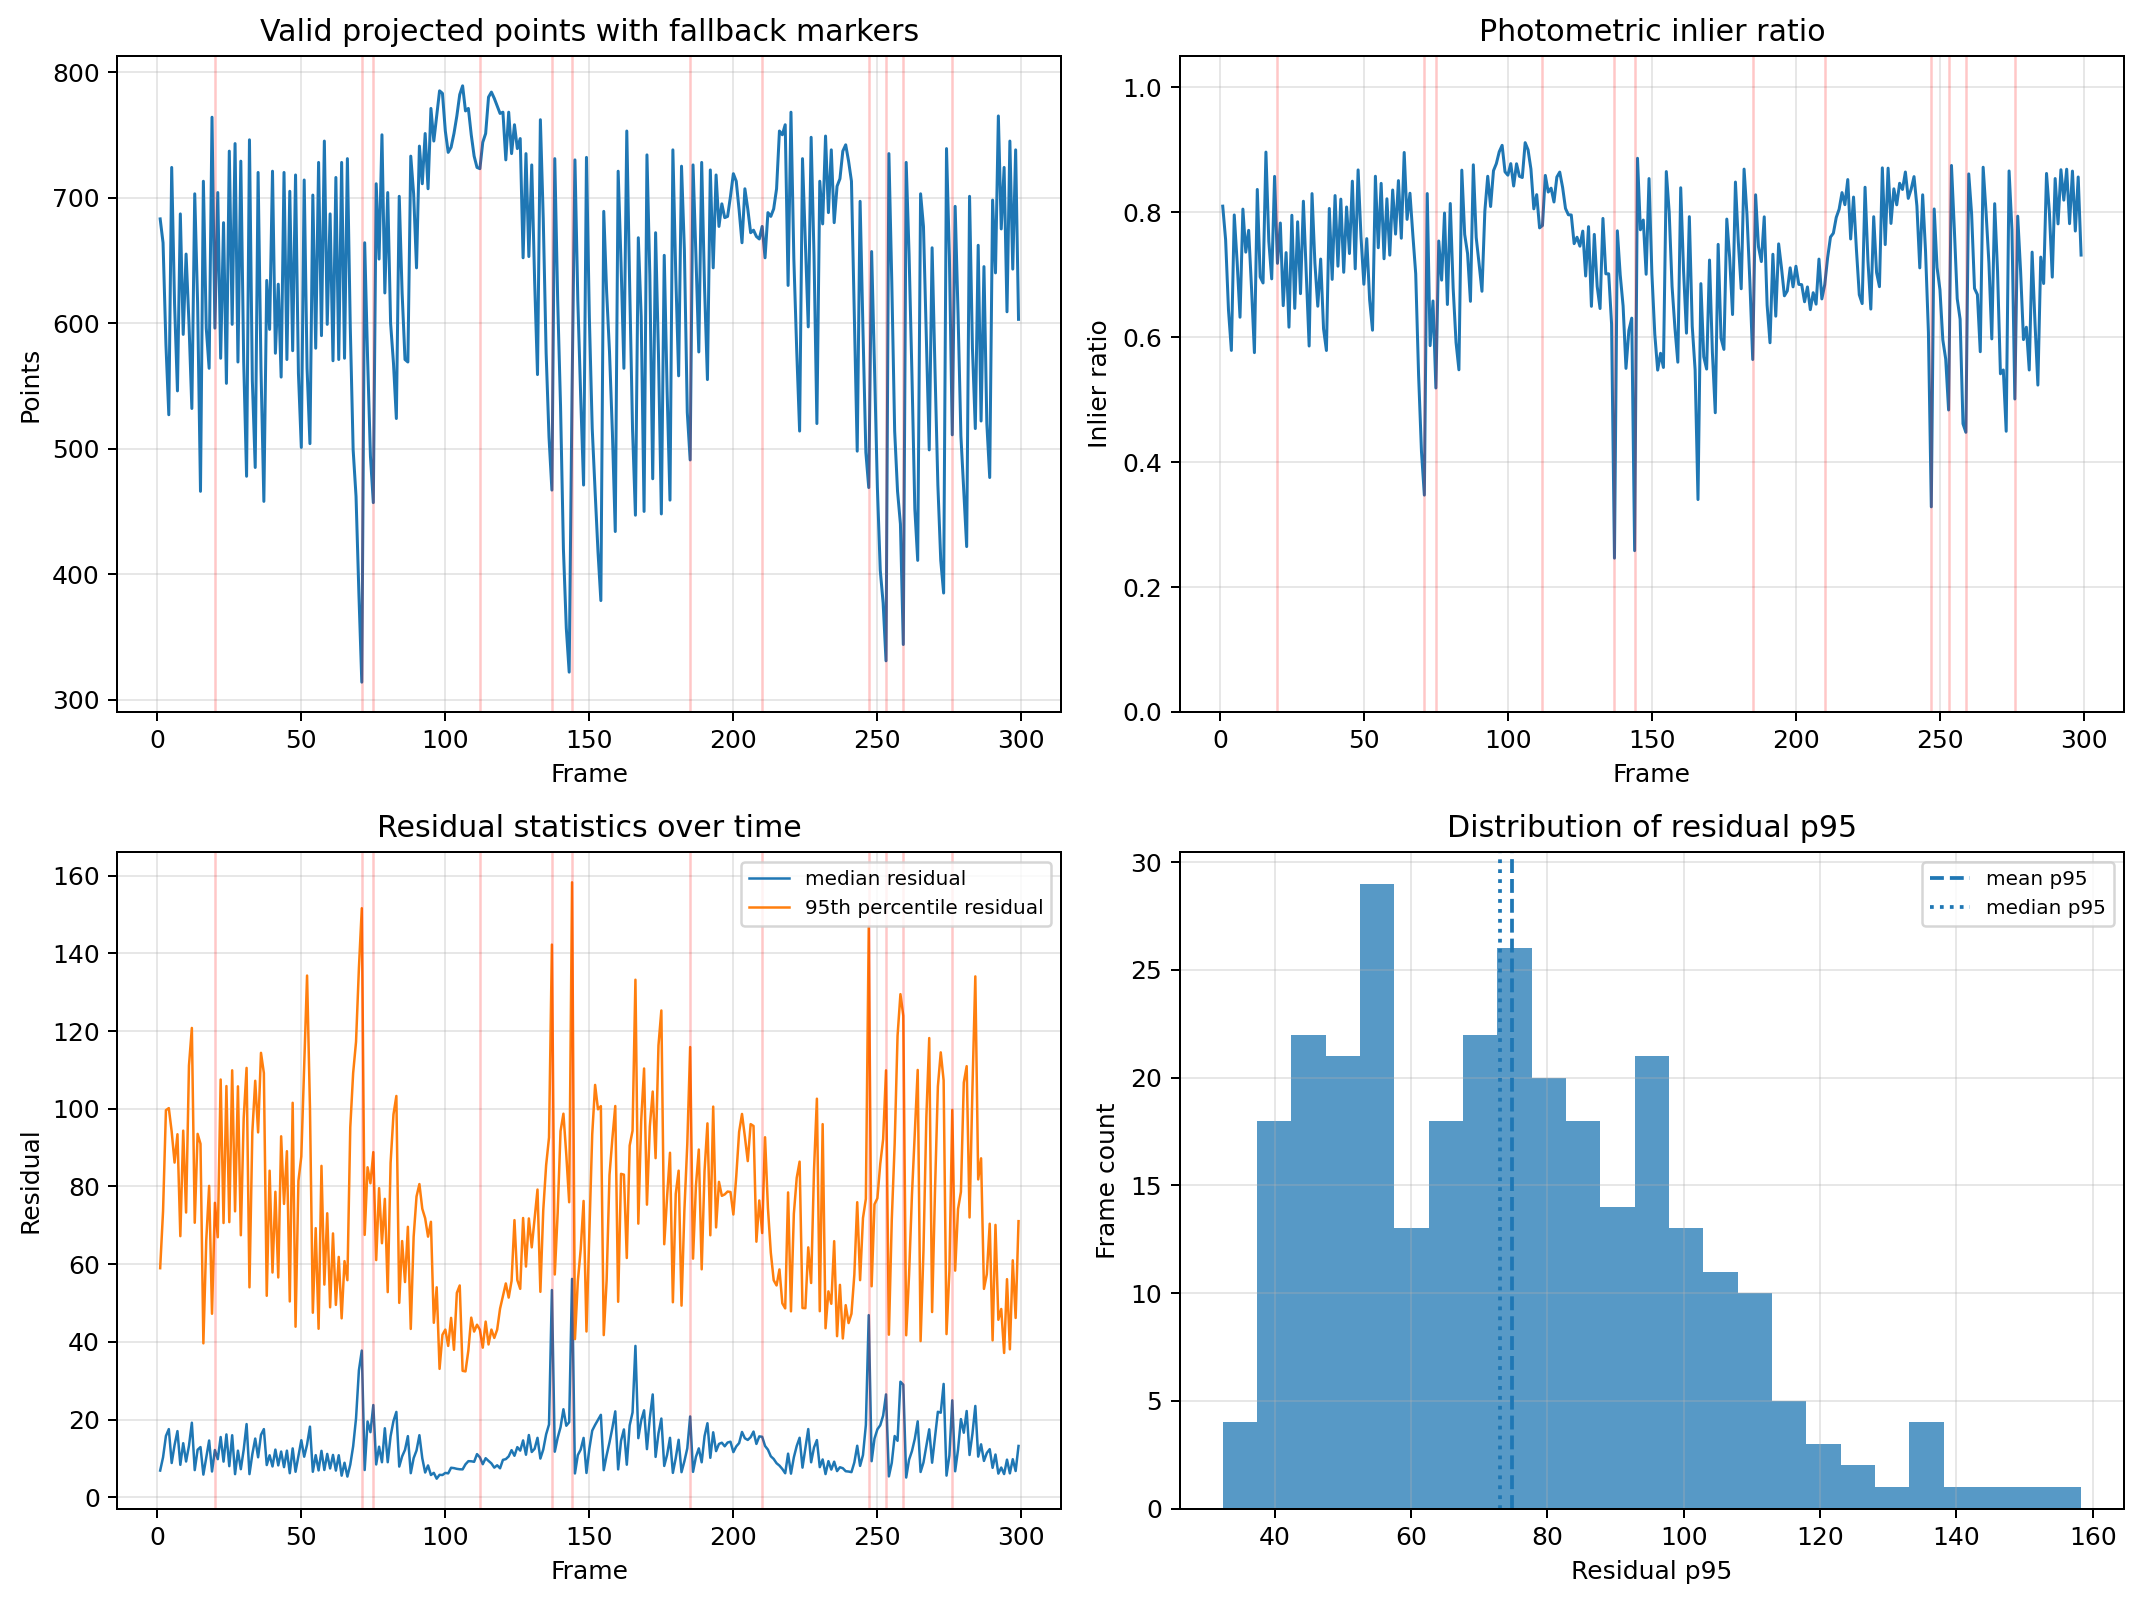
\includegraphics[width=\textwidth]{final300_dso_diagnostics_enhanced.png}
  \caption{Enhanced DSO diagnostics for the final 300-frame optimized run. Red vertical lines mark frames with tracking failure and fallback. The lower-right panel reports the residual-p95 histogram over valid frames.}
  \label{fig:dso-diagnostics-enhanced}
\end{figure}

Figure~\ref{fig:dso-residual-scatter} further relates residual quality to the number of valid projected points. Failure frames are not explained by one scalar threshold alone; rather, they appear in regions where valid projection count, residual p95, LK support, and photometric optimization quality jointly become unreliable. This is why the optimized baseline combines several gates rather than relying on a single rejection rule.

\begin{figure}[H]
  \centering
  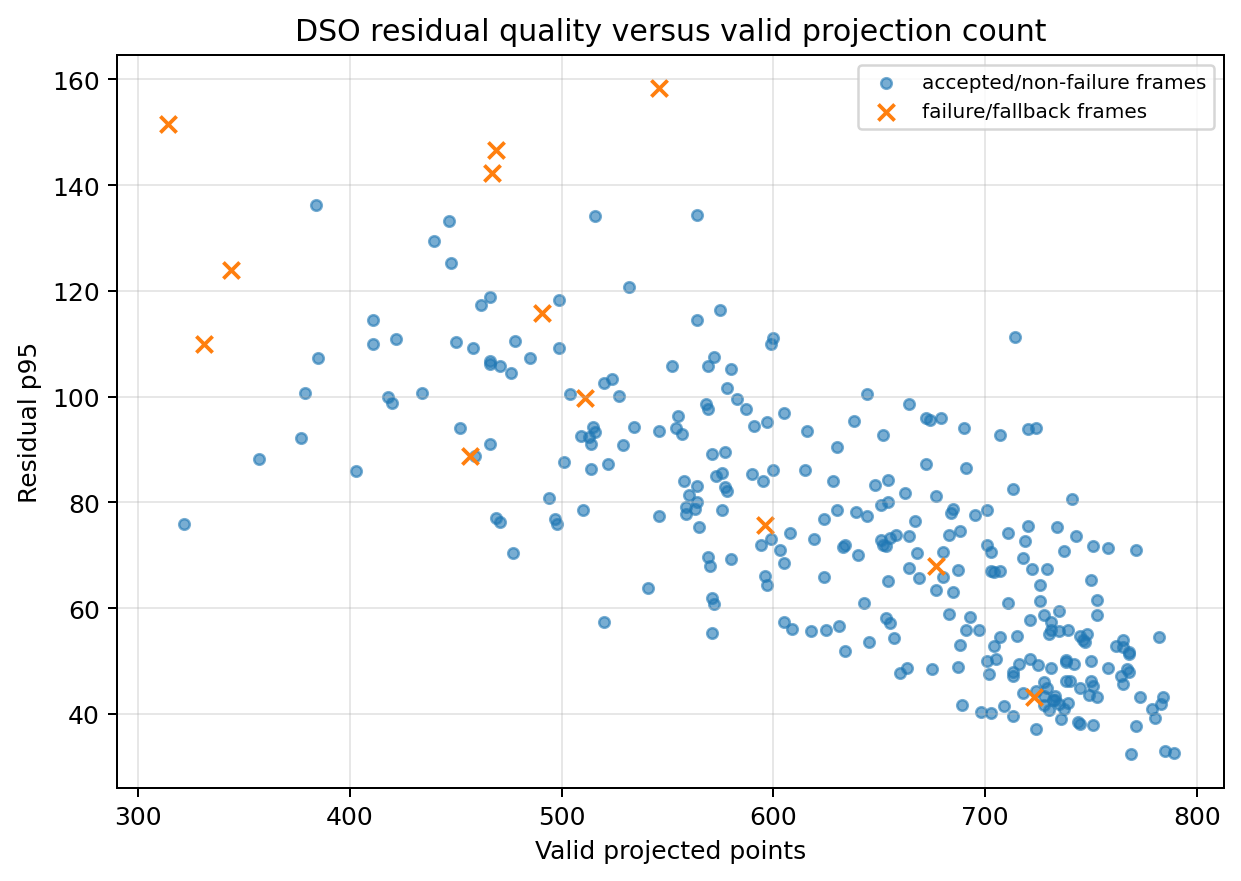
\includegraphics[width=0.72\textwidth]{final300_dso_residual_scatter.png}
  \caption{DSO residual quality versus valid projected point count. Failure/fallback frames are marked separately to show that DSO failure is a multi-factor event rather than a single residual-threshold phenomenon.}
  \label{fig:dso-residual-scatter}
\end{figure}

\FloatBarrier

\subsection{DSO Ablation Study}

The latest DSO ablation is run for 300 frames with 800 sparse points. Table~\ref{tab:dso-ablation} reports accuracy and failure statistics, and Table~\ref{tab:dso-ba-counters} reports selected backend counters. The most decisive result is the \texttt{no\_joint\_ba} configuration: without joint active-window BA, ATE RMSE increases to 59.3614 m and translational RPE increases to 36.0059\%. This is the clearest evidence that active-window optimization is essential in the optimized DSO-style baseline.

Other ablations require careful interpretation. Disabling left-right depth consistency increases ATE from 3.4279 m to 3.7716 m, supporting the usefulness of stereo consistency filtering. Disabling quality gates gives similar ATE, 3.4419 m, but the strict configuration is more transparent because it records controlled rejection semantics. The \texttt{photometric\_with\_motion\_gate} and \texttt{outlier\_culling\_off} configurations obtain lower ATE, 2.8182 m, but they also record 25 failures and 25 fallbacks. Therefore, the lowest ATE alone is not the most reliable selection criterion. The strict full configuration is chosen as the main result because it combines moderate ATE, active-window BA, stereo consistency, strict loop verification, and controlled failure handling.

\begin{table}[H]
\centering
\scriptsize
\caption{DSO ablation accuracy and failure statistics on KITTI sequence 00, 300 frames, and 800 sparse points. These results diagnose the optimized DSO-style baseline and are not claims about full DSO.}
\label{tab:dso-ablation}
\resizebox{\textwidth}{!}{%
\begin{tabular}{lccccc}
\toprule
Configuration & ATE RMSE (m) & RPE t (\%) & RPE r (deg/m) & Failures / fallbacks & Loop candidates / closures \\
\midrule
strict\_full & 3.4279 & 2.0376 & 0.01598 & 12 / 12 & 17 / 0 \\
no\_left\_right\_check & 3.7716 & 2.8142 & 0.02683 & 6 / 6 & 16 / 0 \\
no\_quality\_gates & 3.4419 & 2.0374 & 0.01600 & 11 / 11 & 17 / 0 \\
no\_joint\_ba & 59.3614 & 36.0059 & 0.48667 & 12 / 12 & 17 / 0 \\
no\_affine\_brightness & 3.3253 & 2.0561 & 0.01827 & 7 / 7 & 16 / 0 \\
loop\_candidates\_only & 3.4279 & 2.0376 & 0.01598 & 12 / 12 & 17 / 0 \\
lk\_pnp\_only & 3.7976 & 3.0281 & 0.02031 & 9 / 9 & 15 / 0 \\
photometric\_with\_motion\_gate & 2.8182 & 1.7395 & 0.01473 & 25 / 25 & 16 / 0 \\
grid\_uniform\_selection & 4.0708 & 2.5954 & 0.02641 & 16 / 16 & 13 / 0 \\
outlier\_culling\_on & 3.6680 & 2.1737 & 0.02057 & 17 / 17 & 13 / 0 \\
outlier\_culling\_off & 2.8182 & 1.7395 & 0.01473 & 25 / 25 & 16 / 0 \\
\bottomrule
\end{tabular}}
\end{table}

\begin{table}[H]
\centering
\scriptsize
\caption{Selected DSO ablation backend counters for the 300-frame run.}
\label{tab:dso-ba-counters}
\begin{tabular}{lcc}
\toprule
Configuration & BA accepted / runs / rejected & Active points culled \\
\midrule
strict\_full & 47 / 64 / 17 & 1282 \\
no\_left\_right\_check & 53 / 68 / 15 & 1558 \\
no\_quality\_gates & 48 / 65 / 17 & 1255 \\
no\_joint\_ba & 62 / 64 / 2 & 511 \\
no\_affine\_brightness & 64 / 66 / 2 & 1746 \\
loop\_candidates\_only & 47 / 64 / 17 & 1282 \\
lk\_pnp\_only & 49 / 65 / 16 & 1416 \\
photometric\_with\_motion\_gate & 42 / 59 / 17 & 2480 \\
grid\_uniform\_selection & 47 / 63 / 16 & 1238 \\
outlier\_culling\_on & 46 / 61 / 15 & 2582 \\
outlier\_culling\_off & 42 / 59 / 17 & 2480 \\
\bottomrule
\end{tabular}
\end{table}

Figure~\ref{fig:dso-ablation-enhanced} visualizes the same ablation evidence. The large ATE bar for \texttt{no\_joint\_ba} makes the role of active-window refinement immediately visible. The failure/fallback panel also shows why ATE alone is insufficient: some low-ATE configurations rely on many more fallback events. A stronger system should optimize both trajectory error and failure frequency.

\begin{figure}[H]
  \centering
  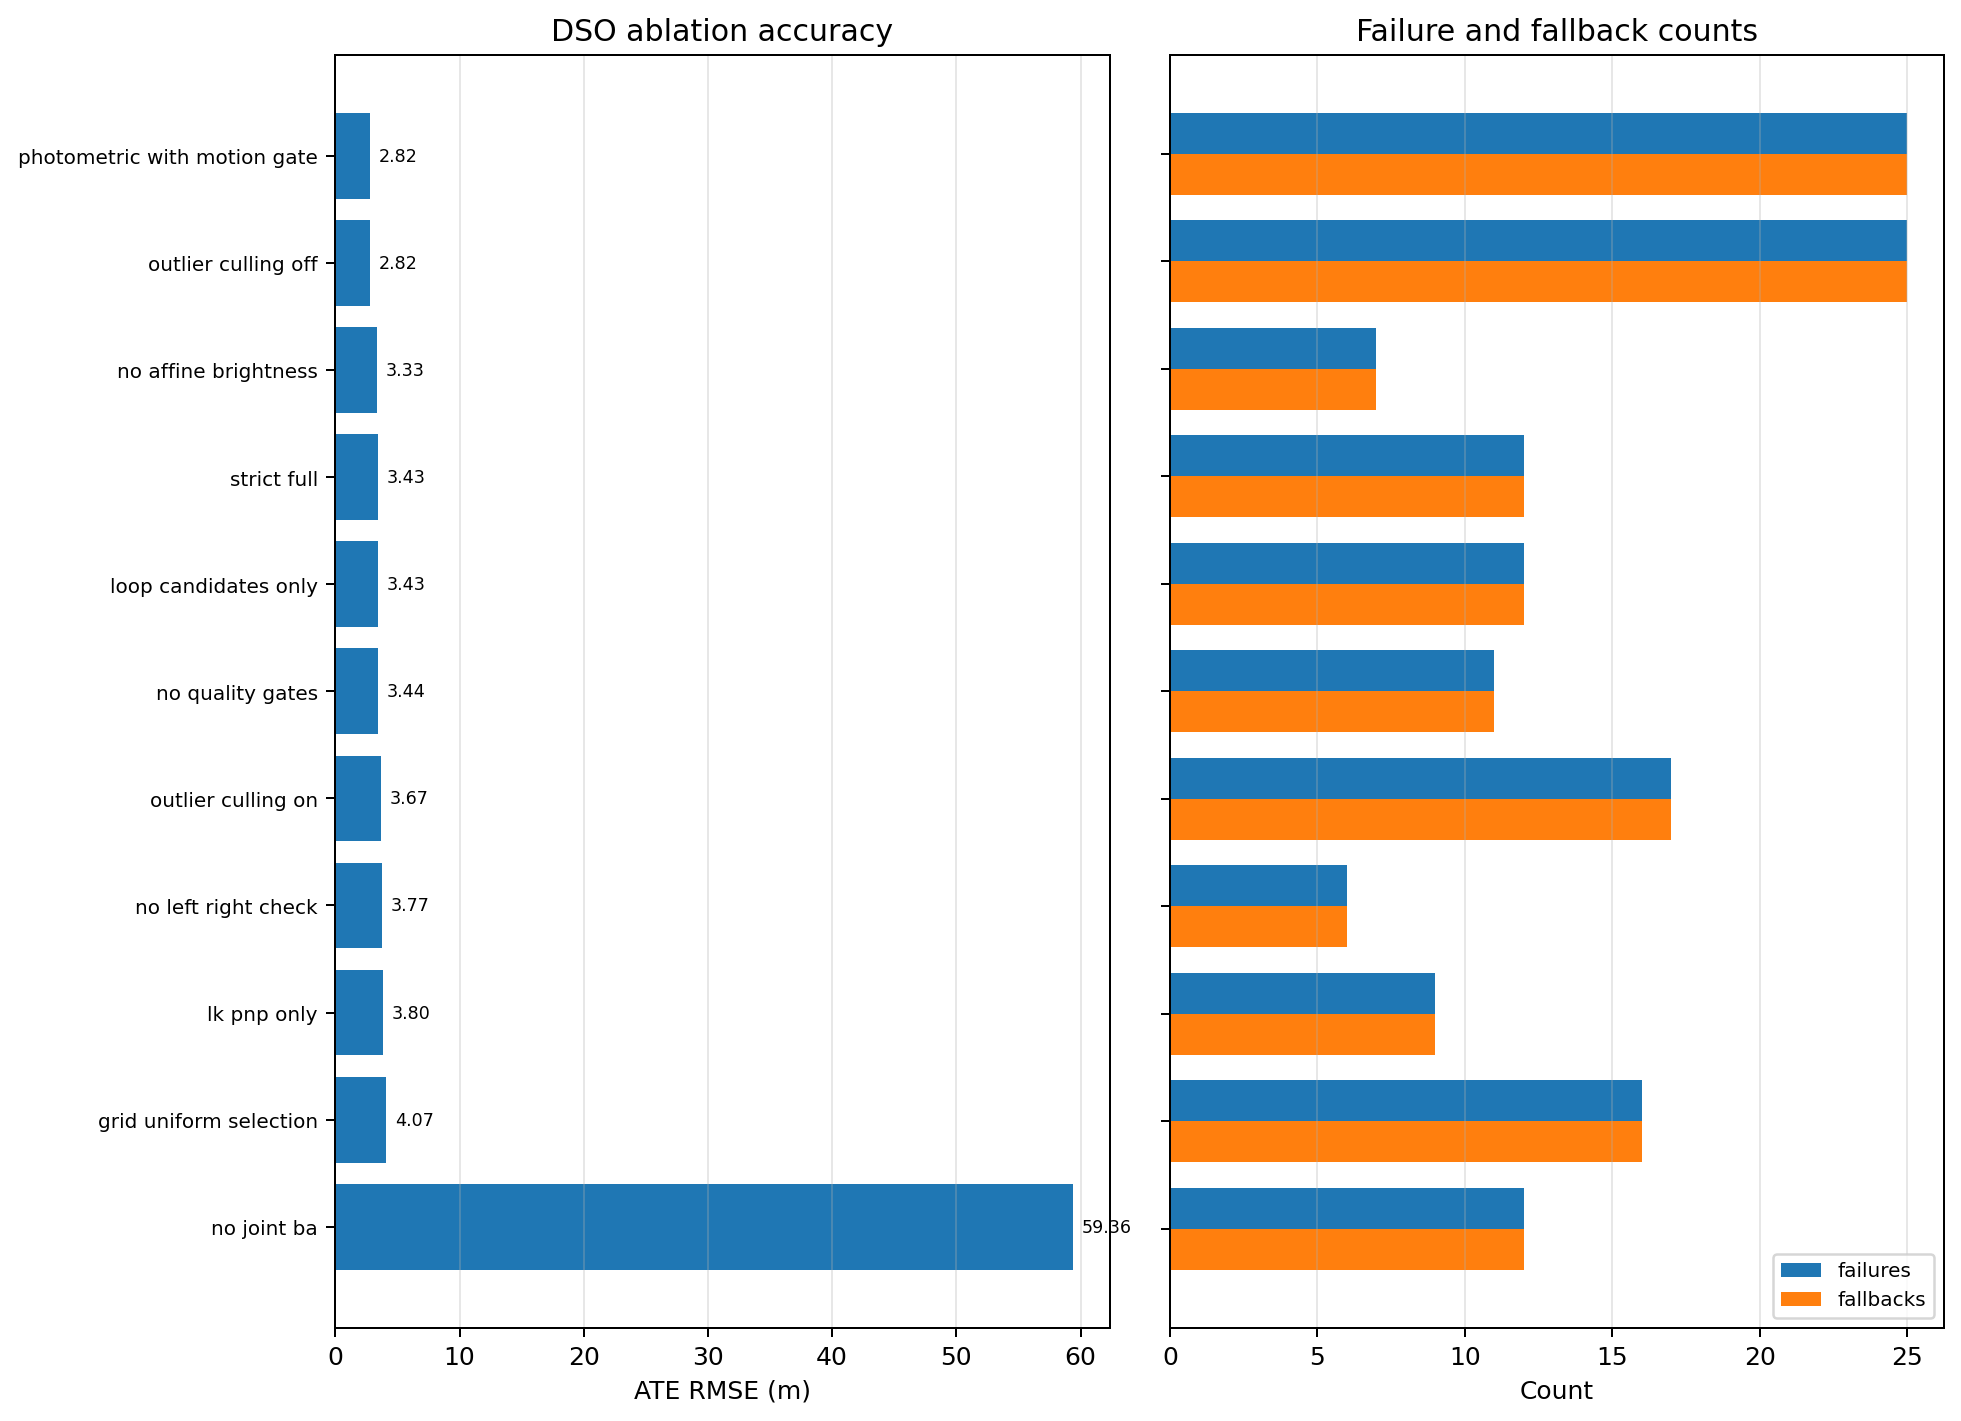
\includegraphics[width=\textwidth]{dso_ablation_300_enhanced.png}
  \caption{Enhanced DSO ablation plot for the 300-frame, 800-point experiment. The left panel reports ATE RMSE, sorted by ATE; the right panel reports failures and fallbacks.}
  \label{fig:dso-ablation-enhanced}
\end{figure}

\FloatBarrier

\subsection{Analysis and Threats to Validity}

The 300-frame experiment changes the interpretation of the project. In the earlier 100-frame report, the DSO-style baseline remained far behind ORB and SVO. After additional stabilization and the 300-frame rerun, the optimized DSO-style baseline is much closer to the other two methods: 3.4279 m ATE compared with 2.9913 m for ORB and 2.9621 m for SVO. DSO also obtains lower translational RPE than ORB in this run. This indicates that the new DSO components are not merely cosmetic diagnostics; they materially improve the direct sparse baseline.

The SVO-style baseline has the best speed-accuracy trade-off in the final run. It obtains the lowest ATE, the lowest translational RPE, the lowest KITTI translational segment error, and by far the lowest runtime. This supports the semi-direct design rationale. Optical-flow or patch-based tracking avoids the cost of full descriptor matching, while PnP RANSAC still supplies geometric pose estimation. The cost is that the current SVO-style baseline lacks loop closure and maintains many keyframes.

The ORB-style baseline remains robust. It completes the 300-frame run with zero tracking failures and records two loop closures. Its high p95 runtime, however, shows that the Python implementation sometimes invokes expensive feature, local map, or loop-related operations. This should not be interpreted as the runtime of official ORB-SLAM2; it is a property of this Python baseline.

The optimized DSO-style result must be interpreted carefully. It does not show that direct methods are worse than feature-based or semi-direct methods. Instead, it shows that a simplified Python direct sparse baseline can become competitive when active-window BA, left-right depth consistency, point culling, strict loop semantics, affine brightness handling, and fallback are added. Its remaining 12 failures indicate that photometric tracking is still sensitive to initialization, residual quality, and point lifecycle management.

The main threats to validity are as follows. First, the final evaluation uses only KITTI sequence 00, so the conclusions may not generalize to other motion patterns, scene structures, or lighting conditions. Second, the 300-frame subsequence is more informative than the earlier 100-frame run but is still not a complete KITTI sequence evaluation. Third, backend maturity differs across baselines; therefore, the comparison is not a ranking of the original algorithm families. Fourth, hardware specifications were not logged, so runtime values are local measurements rather than portable benchmarks. Fifth, loop-closure behavior remains limited: ORB records two closures, DSO records candidates but no verified/corrected closures, and SVO has loop closure disabled. The experiments therefore emphasize odometry and local-SLAM behavior more than mature long-term loop correction.

\section{Research Conclusions}

This project implements and compares three Python visual SLAM/VO research baselines on KITTI Odometry: \methodorb{}, \methoddso{}, and \methodsvo{}. The final 300-frame experiment on KITTI sequence 00 shows that the SVO-style baseline achieves the lowest ATE RMSE of 2.9621 m, the lowest translational RPE of 1.7526\%, and the lowest runtime. The ORB-style baseline obtains a very similar ATE RMSE of 2.9913 m with zero tracking failures, but it is much slower in this Python implementation. The optimized DSO-style baseline obtains 3.4279 m ATE RMSE and records 12 failures and 12 fallbacks, yet it is much closer to the other two baselines than the earlier simplified direct sparse result.

The most important conclusion is that frontend design, point selection, residual modeling, active-window optimization, and failure-handling policies jointly determine SLAM behavior. In the latest data, the semi-direct SVO-style baseline provides the strongest speed-accuracy compromise. The ORB-style baseline remains robust but computationally expensive. The optimized DSO-style baseline demonstrates that direct sparse tracking can be substantially improved by adding strict loop verification, stereo consistency filtering, active-window BA, affine brightness handling, point lifecycle controls, and transparent diagnostics.

The DSO ablation study is especially informative. Disabling joint active-window BA causes the largest degradation, increasing ATE to 59.3614 m. Some configurations obtain lower ATE than the strict full setting but also introduce many more fallback events. Therefore, a reliable SLAM baseline should be judged by accuracy, robustness, backend counters, and failure semantics together. These conclusions apply only to the implemented Python research baselines and are not claims about the full official ORB-SLAM2, DSO, or SVO systems.

Future work should evaluate additional KITTI sequences, log complete hardware and software environment details, run full-sequence experiments, strengthen the photometric backend, improve mature relocalization and loop closure, and compare against official C++ and modern deep SLAM systems under clearly separated protocols.

\section{Personnel and Task Division}

\begin{table}[H]
\centering
\caption{Personnel and task division.}
\label{tab:personnel}
\begin{tabular}{ll}
\toprule
Personnel & Task division \\
\midrule
24376333 Huang Yibo & Algorithm implementation and paper writing \\
24376267 Wang Xihao & Algorithm execution and checking; reference preparation \\
24301017 Yang Xiaochu & Experimental data preparation \\
\bottomrule
\end{tabular}
\end{table}

\renewcommand{\refname}{8 References}
\bibliographystyle{ieeetr}
\bibliography{references}

\end{document}
